\chapter{Related Work}
\todo: remake description! \\
Define study parameters by analysing related work.
%In chapter 2 A1, A3, A4, A6, A7, A10, A14 and 15 are already discussed. In this chapter the remaining aspects are analysed by investigating how other researchers decided on them. The remaining aspects are dependent variables (A2), the task (A5), the MR technology to use (A8), the tracking technology (A9), the behaviour of the instructions (A11), the measures to apply (A12) and the considered body parts (A14). These aspects are better discussed at existing systems to make sure the study having a high validity. This chapter is structured by means of the perspective though the independent variables, namely ego-centric, exo-centric and the combination of both. In this subchapters the aspects are discussed and concluded. In the overall conclusion a decision is made for the aspects by comparing them to each other. eg, the task must be suitable for all perspectives.

\section{Overview}
Table \ref{tbl:overviewTable} shows previous work of researchers connected with motor learning in MR. In total there five classes of tasks they used for evaluation. The most common task is \textit{arts}, like Martial Arts or Tai Chi \cite{Han2016}, \cite{Yan2015}, \cite{Katzakis2017}, \cite{Han2017}, \cite{Portillo2008}, \cite{Hoang2016}, \cite{Chua2003} \cite{Anderson2013a}
\begin{table}
	\centering
	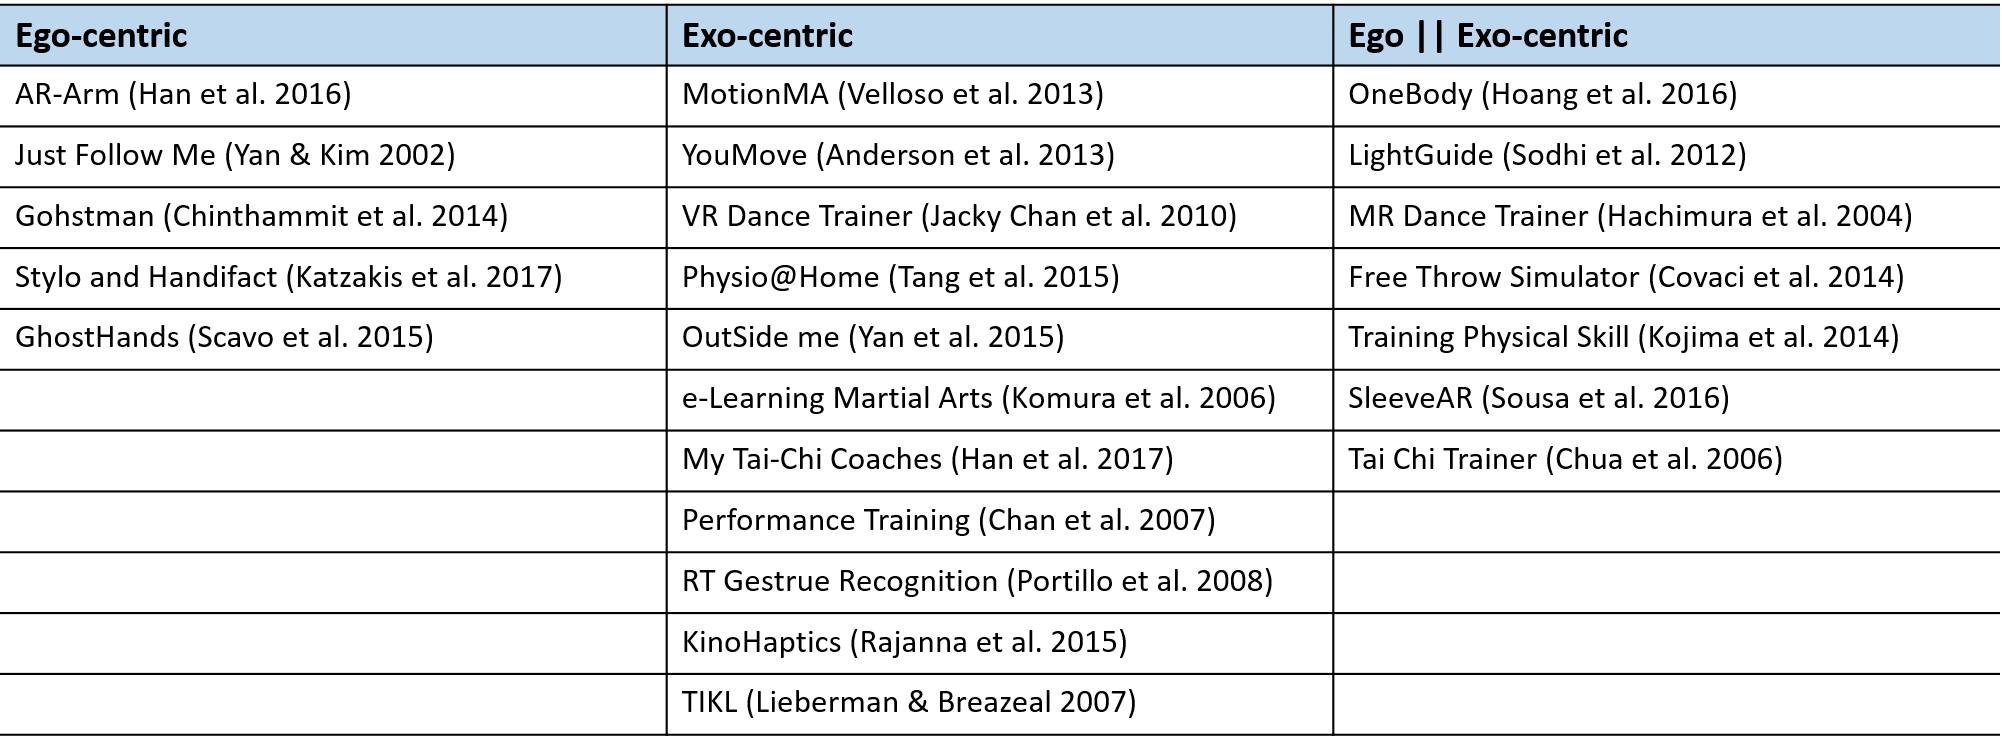
\includegraphics[width=1.0\textwidth]{img/overview_table.png}
	\caption{overview all papers \todo ref as table}
	\label{tbl:overviewTable}
\end{table}
\begin{table}
	\centering
	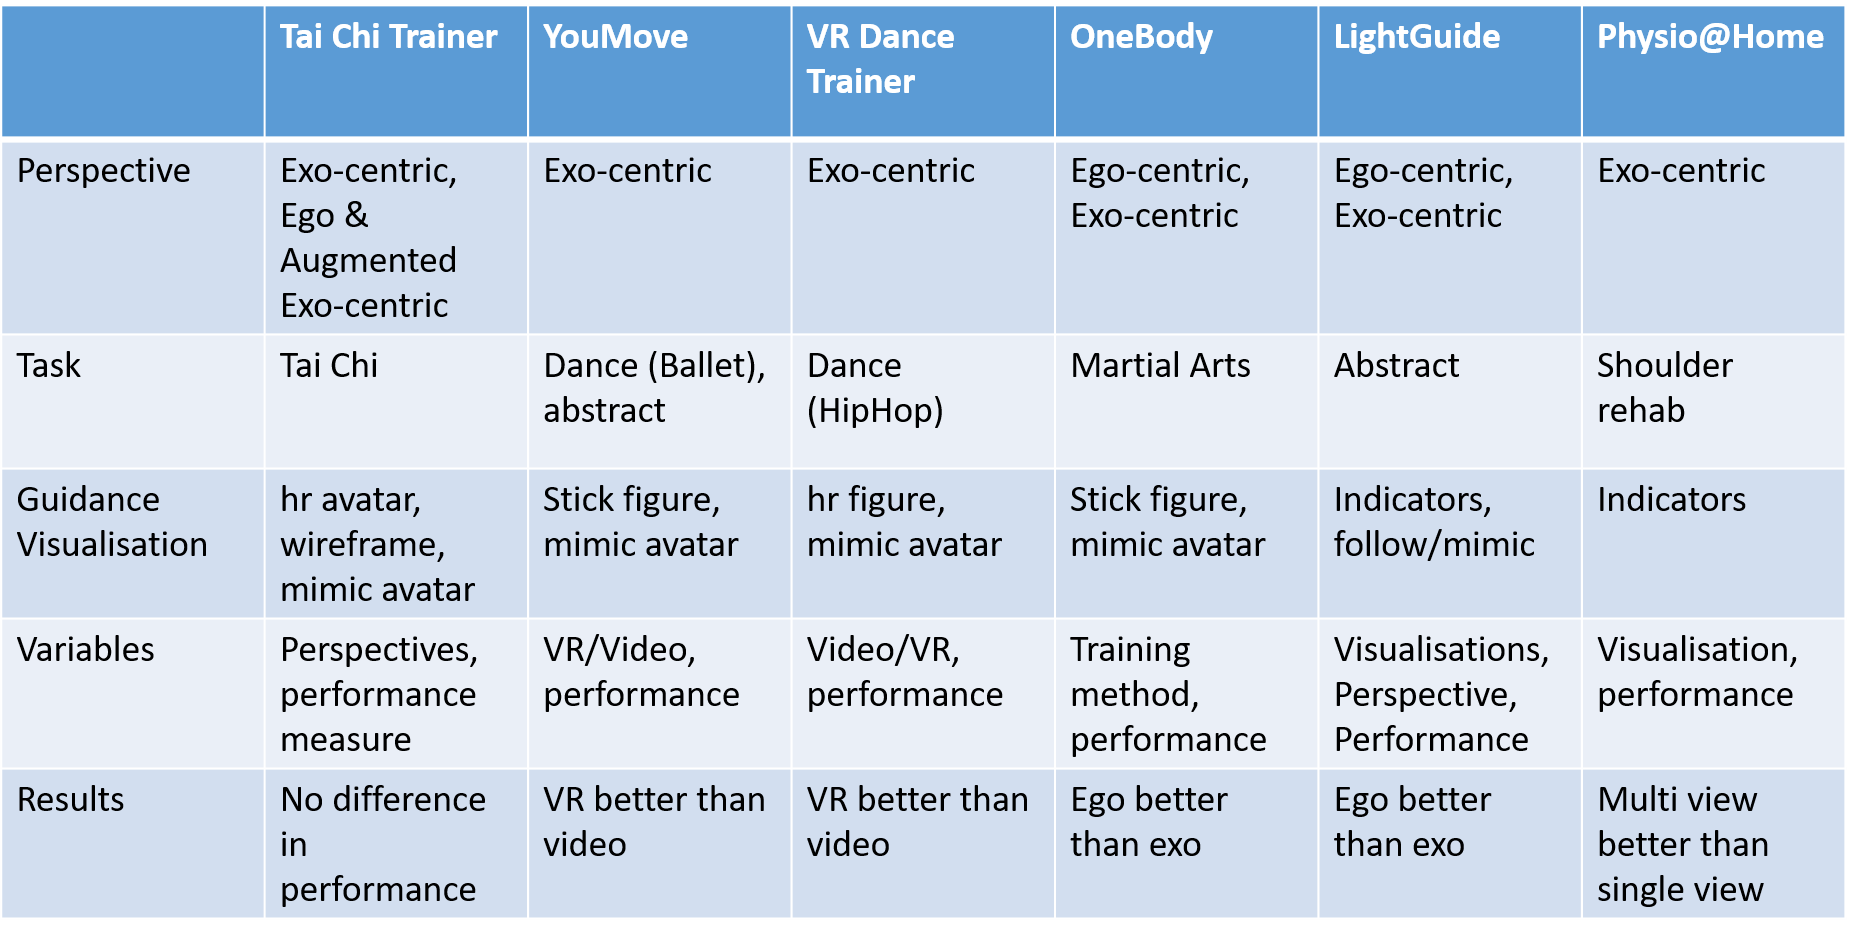
\includegraphics[width=1.0\textwidth]{img/detail_paper_overview.png}
	\caption{detail paper overview \todo ref as table}
	\label{tbl:detailOverviewTable}
\end{table}


\section{Analysis}
\subsection{Implemented Visual Perspective}
%how are they implemented and technology
%---
Chua et al. \cite{Chua2003} implemented five different perspectives to teach with \textbf{Tai Chi Trainer}, compare \ref{fig:taichiperspectives}. There are three exo-centric perspectives (a-c, further called conditions a-c) and two ego-centric perspectives combined with exocentric (d,e, further called conditions d,e). In \textbf{One on One} the student stand next to one teacher, which is closest to a real world training scenario \ref{fig:taichiperspectives}(a). In con \--- \textbf{Four Teachers} \--- the student is surrounded by four teachers, with the student in the middle \ref{fig:taichiperspectives}(b). The \textbf{Side by Side} \ref{fig:taichiperspectives}(c) condition shows four pairs of teacher and student in the same formation as in condition (b). The first ego-centric \& combined condition is called \textbf{Superimposition 1} \ref{fig:taichiperspectives}(d). Here the formation still remains, but the student in the middle is surrounded by four more students. On each of the student a red wireframe teacher is superimposed. \textbf{Superimposition 2} \ref{fig:taichiperspectives}(e), is similar to Superimposition 1 and differs only in the visual representation: the student is now a green, transparent wireframe. Chua et al. use no pure ego-centric perspective, since in the latter two conditions the teacher can be seen also from the exo-centric perspective.
\begin{figure}
	\centering
	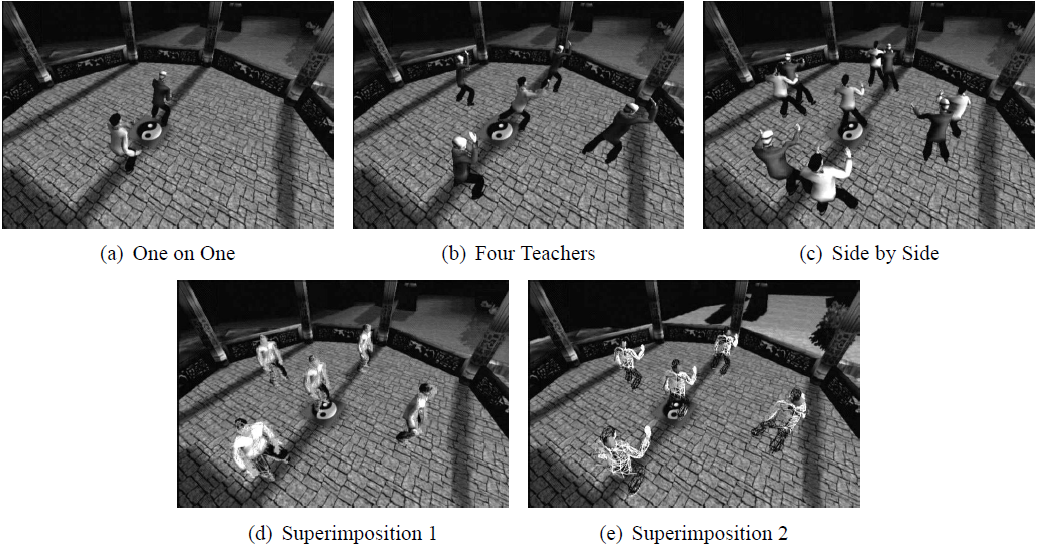
\includegraphics[width=1.0\textwidth]{img/taichi_perspectives.png}
	\caption{Used perspectives at \cite{Chua2003}}
	\label{fig:taichiperspectives}
\end{figure}\\
%---
$ $\\
\textbf{YouMove} uses Microsoft Kinect (\todo ref) to record motions and to track the student. The recorded instruction as well as the students movements are projected on an AR mirror. The special about this mirror is, that the degree of reflection can be changed by simply adjusting the light in the room. With this, the student can see his own real body as reflection as well as the projection of a beamer simultaneously. If the room is bright, the student sees only his reflection and in a dark room only the projection is visible.\\ 
YouMove provides multiple stages for the learning process: (1) Demonstration, (2) Posture Guide, (3) Movement Guide, (4) Mirror, (5) On your own. In stages 1-3, the student sees the guidance visualisation in the exo-centric perspective. In (1) the user sees a video of the movement. In stage 2 \& 3 the user is superimposed by a skeleton. Stage 4 \& 5 does not allow a view on the teachers representation. After each stage a feedback is given. This view provides multiple views for the four keyframes: a skeleton of the teacher and student superimposed, a video of the teachers demonstration and a video of the moves of the student.\\ \\
%---
\textbf{VR Dance Trainer}. Chan et al. \cite{Chan2011a} facilitate a 3D screen for rendering the avatars. The student is tracked by an optical motion capturing system. In the first phase (demonstration) only the teacher is shown on the screen. In the second phase (practise) teacher and student can be seen simultaneously, standing side by side. Additionally, both avatars are mirrored, so the exo centric viewer can observe the avatars from back and the front at the same time, compare figure \ref{fig:vrdt}. In the final phase (feedback) the student sees the teacher and the students performance in slow motion side by side.\\ \\
%---
\textbf{LightGuide} \cite{Sodhi2012} achieved an ego-centric guidance without using a HMD. The student stands under a depth camera and a projector. The depth camera tracks the hand of the student. This position is utilised and the guidance visualisation is projected directly on the users hand. During the evaluation of the system, four conditions used this ego-centric position. The remaining conditions shown exo-centric on a screen or directly on the hand.\\ \\
%---
\textbf{Onebody} \cite{Hoang2016} show the guidance visualisation in an ego-centric perspective, too, but with an HMD. The teacher is projected inside the body of the student. Both, teacher and student are tracked by skeletal tracking, using a Microsoft Kinect \todo. The visualisation of the teacher is attached to the hip of the student. To overcome different body sizes, the avatars are normalised and scaled to the size of the student. For a second condition an exo-centric view is provided with a HMD, too. There the teacher stands in front of the student.\\ \\
%---
\textbf{Physio@Home} by Tang et al. \cite{Tang2015} used a Microsoft Kinect in combination with a screen forming together an augmented reality mirror. The participant stands in front of the screen and is tracked by the Kinect. On the screen the participant is augmented by moving instructions. The perpective on the guidance visualisation is exo-centric. Tang et al. faced the problem, that the front facing projection lacks of 3D queues. Their solution was the multi camera views. A second view is provided from above, aiming to help the participant to maintain a correct angle of the arm. In the study, four conditions were examined: videoSingle, videoMulti, wedgeSingle and wedgeMulti. Here, video and wedge indicate the guidance visualisation, single and multi indicate the numbers of visualisations.
%---
%---
%how are they implemented and technology
\subsubsection{Conclusion}
There are multiple ways of realising ego-centric, exo-centric or combination perspectives on guidance visualisations. Ego-centric views are realised through superimposition of the teacher and the student like seen in Tai Chi Trainer and OneBody or projected movement instructions directly on the student like in LightGuide. The first two use an HMD to realise the ego-centric perspective. For the exo-centric perspective more possibilities exist like an augmented reality mirror (YouMove), screens or 3D screens (Tai Chi Trainer, Physio@Home) or projectors (LightGuide). Exo-centric perspective can also be achieved with HMD's (OneBody, Tai Chi Trainer). One main benefit of HMD's is the easy visualisation of ego-centric and exo-centric perspectives simultaneously. Because of this I decide to use an HMD for my study. The Tai Chi Trainer achieved the simultaneous perspective by placing the teacher inside the student and outside the student, but did not achiev any significant differences in learning performance; but this could be overcome by today's technology. This representation is chosen for the study. In addition, the authors of the paper state the importance of multiple view (Physio@Home, Tai Chi Trainer, YouMove), if the avatar is rendered on 2D screens, because of missing 3D queues. This can be partly overcome within a VE. But to provide multiple angles on the guidance visualisation could still be necessary. Therefore I decide to let the student moving freely around the guidance visualisation. Since other factors like feedback play also a role for the perspective, the exact definition of the perspective to implement is given in the conclusion of this chapter.



\subsection{Study task}
%only Task
%---
The task in Chua's \cite{Chua2003} \textbf{Tai Chi trainer} is \--- as the name indicates \--- a Tai Chi motion. A professional Tai Chi trainer was invited to perform a so called \textit{Tai Chi form} and recorded offline. This \textit{form} was segmented in four ca. 20 seconds long sequences (Motion 1-4). "Motion 1 featured simple hand movements and a 90 degree turn to the right; motion 2 had little hand motion, a 180 degree turn of the feet, and some turning of the upper body; motion 3 featured slow hand motions, large movement of the feet, and some turning of the thorax; and motion 4 featured swift hand movement and turning of the thorax and hips but little movement of the feet." \cite{Chua2003}. Error measurements indicated that all motion but motion 1 had the same difficulty, being significantly easier. This movements can be classified as \textit{sequential movements} according to chapter 2 \todo ref. 40 volunteers conducted the movements in a study to evaluate their system. They randomized the condition (described in next chapter, compare figure \ref{fig:taichiperspectives} condition a-e) and the motion to minimize learning effects. For each motion and condition pair, the Tai Chi student were asked to match the Tai Chi teachers demonstration during twelve repetitions.\\ \\
%---
\textbf{YouMove} by Anderson et al. \cite{Anderson2013a} is a movement training system, suitable for a vast range of moves. A movement can be recorded and then edited by an authoring tool. After the editing, the movement is added to the internal library, from which it can be chosen by a student. For the study itself, an author or the paper \--- though no professional \--- recorded four movements. Two of them from ballet and two abstract movement. The authors decided to variate the difficulty of the task, namely "the ballet movements [...] were easier to conceptualise and required only moderate movement.", while "the abstract movements were more difficult to perform, as they were a series of postures with no clear structure and required substantial movement." The movements consisted of four keyframes. Keyframes are important points during the movements, determined and set by the person recording a movement.\\ \\
%---
Jacky Chan et al. developed a \textbf{VR Dance trainer} \cite{Chan2011a}. For their system they invited professional Hip-Hop dancers and recorded their movements. The learner of the movement can choose a movement out of a database. One movement lasts around 2 seconds. First, the teacher appears and the student watches the demonstration, while he can adjust the demonstration speed and viewpoint. After that, the student practices the dance moves by mimicking the teachers avatar. Finally the student can see a slow motion replay of the performance. One hole session takes 15 minutes.\\ \\
%---
In contrast to all other systems, \textbf{Lightguide} by Sodhi et al. \cite{Sodhi2012} build on abstract movements to evaluate their system. Sodhi et al. focus on single arm movements, directed by an guidance visualisation on the hand. The participants perform five movements, namely a line, a "N", a square, a circle and a bowed line, compare figure \ref{fig:lightguide1} left. All movements were performed in three different angles, like shown in figure \ref{fig:lightguide1} right.
\begin{figure}
	\centering
	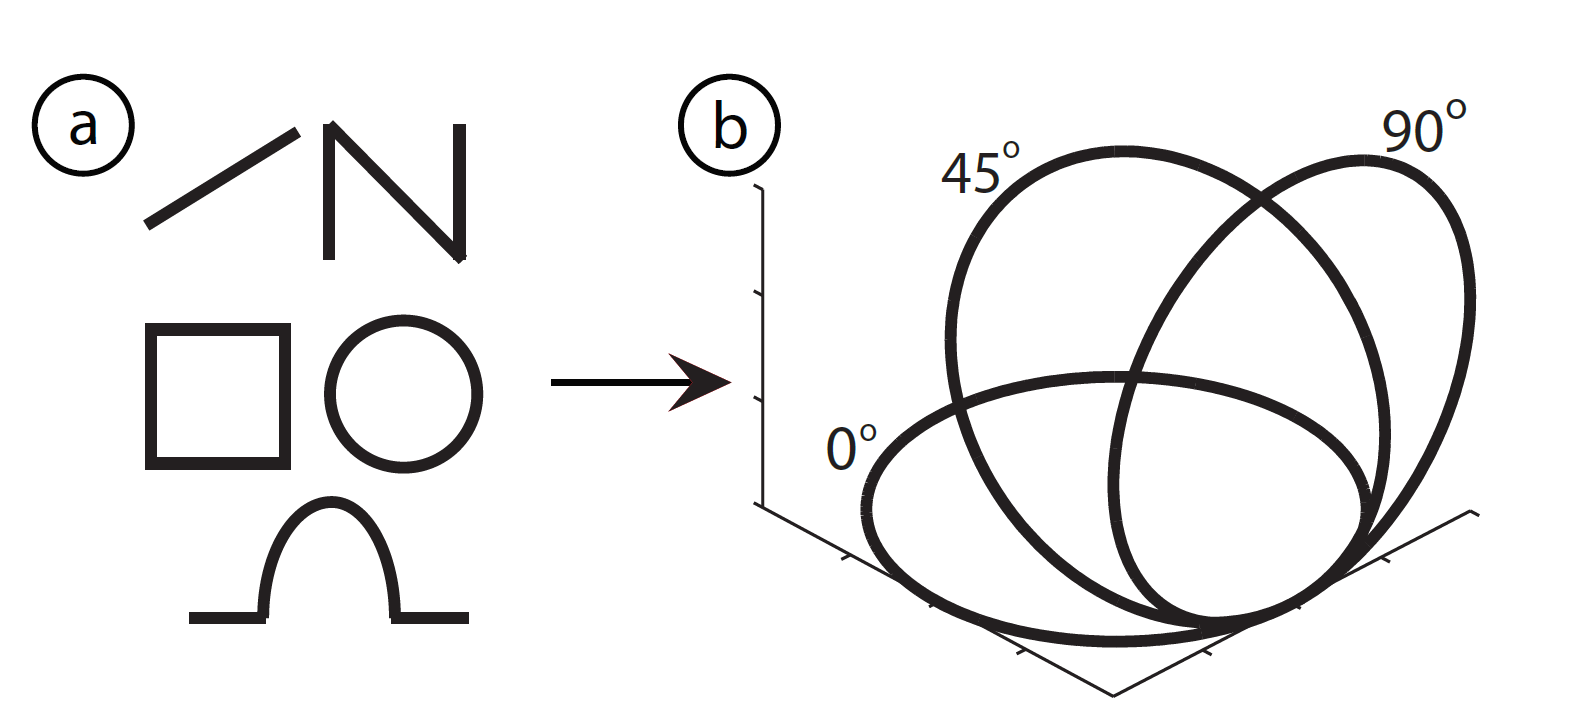
\includegraphics[width=1.0\textwidth]{img/lightguide_movements.PNG}
	\caption{movements by lightguide \cite{Sodhi2012}}
	\label{fig:lightguide1}
\end{figure}\\
\todo These movements were performed with six conditions resulting in 90 dataset per participant (6 conditions x 5 path x 3 angles).\\
%---
$ $\\
\textbf{Onebody} by Hoang et al. \cite{Hoang2016} is designed for sports or physical activity training like yoga, dance or martial arts. For the study they used a Martial Arts movement. Each participant started with a training session in which a remote instructor teaches a posture physically and verbally. Verbal feedback was given and the training repeated until the student was confident. After that the final posture was recorded. This applied for four postures with different complexities.\\ \\
%---
\textbf{Physio@Home} by Tang et al. \cite{Tang2015} aim to support rehab exercises for patients at home. Tang et al. chose the shoulder segment as study object, because particpants could do this movement easily while standing, and the ball-socket joint gives more dofs than eg. the knee. In the study itself, 4 tasks had to be completed: straight, angled, elbow and combo.
\begin{itemize}
	\item[straight] "Abduction of arm along the frontal plane up to shoulder level, followed by adduction of arm back to the participant’s side. This is a simple frontal plane exercise.
	Angled."
	\item[angled] "Abduction of the arm at $45^\circ$ from the frontal plane, followed by adduction back to the side. This is an angled variation of the Straight exercise, where interpreting the angle may be difficult."
	\item[elbow] "External rotation of forearm away from the center of the participant’s body until $90^\circ$ from the sagittal plane, followed by an internal rotation back to center. This exercise requires the participant to keep their elbow tucked against their side and is a difficult exercise to understand without depth cues (i.e., with just a frontal view)."
	\item[combo] "Abduction of the arm along the frontal plane up to shoulder level, internal rotation of the arm until pointing forward, followed by an external rotation of the arm back to the frontal plane, and adduction of the arm back to the participant’s side. This is a more complex exercise than the previous three, involving many components."
\end{itemize}
%---
%---

\subsubsection{Conclusion}
As we see in this section, there is a verity of tasks to evaluate movement learning. Namely a Tai Chi form (Tai Chi Trainer \cite{Chua2003}), dance movements (YouMove \cite{Anderson2013a} and VR Dance Trainer \cite{Chan2011a}), physiological rehab movements (Physio@home \cite{Tang2015}), abstract movements (YouMove, LightGuide \cite{Sodhi2012}) and Matial Arts (OneBody \cite{Hoang2016}). For the latter is to mention that the evaluation aimed for postures and not movements. To gain valid data some choose to have tasks with comparable complexity (\cite{Chua2003}, \cite{Anderson2013a} inside Ballet tasks and inside abstract tasks, \cite{Sodhi2012}), therefore eg. one Tai Chi form was taken and split into four sub forms. Physio@home and YouMove (between ballet and abstract) chose to have different complexities of tasks. All but Tai Chi Trainer proofed to be valid for evaluation of movements. But the authors of Tai Chi Trainer see the reason in the hardware performance, what could be overcome with today's technology. All systems but LightGuide aim to be a teaching system for real world tasks. The aim of this thesis is to evaluate the influence of the perspective on guidance visualisations itself, though, both tasks \--- abstract and real world tasks \--- seem suitable for our system. Max, hier dann entscheiden ob was für tasks.


\subsection{Guidance visualisation}
%visual appearence --- shape and colour
%gudance technique
%feedback
%realism degree
Chua's \textbf{Tai Chi training} scenario takes place in pure VR using a HMD. The lessons are conducted in a virtual pergola standing in a nature or park environment. In condition a to c (compare \ref{fig:taichiperspectives}), the student and the teacher are rendered as non transparent, high realism degree avatars. However, in condition d and e, the visual appearance changes. In condition (d) the student is still rendered normally but the teacher is now represented as a red wireframe. Condition (e) was introduced late in the development of the system based on early subject feedback. The students here are rendered as green wireframe avatars and the teacher as red wireframe avatars.\\
In terms of guiding technique, the student is presented the pre recorded motion of the teacher. The teacher avatar performs the motion in question and the student tries to mimic this motion. During the mimicking process no feedback is provided to the student. But in condition (d) and (e) the teacher is superimposed on the students avatar. This can be interpreted as feedback since the difference between the students e.g. arm position and the teachers arm position can be seen easily.\\ \\
%---
The visualisation of the teacher in \textbf{YouMove} is rendered in a low degree of realism \--- only a stick figure in yellow. During the feedback screen after each stage, the student is also rendered as a stick figure but in blue. For teaching, YouMove utilise the above mentioned five training stages. In the first stage (Demonstration), a video of the teacher performing the movements is shown. The student only sees the video and not the reflection of the own body. The second stage (Posture guide) a video and the stick figure of the student are shown, but still not the own reflection. The student is asked to match they postures at specific keyframes, where the demonstration stops. After matching the posture of a keyframe, the demonstration moves on to the next keyframe. In the third stage (Movement Guide) the demonstration no longer stops at the keyframes. Furthermore, the reflection and the projection are visible simultaneously, the student is superimposed by the teachers stick figure. (\todo change skeleton to stick figure). Stage four (Mirror) is like the name indicates: the student stands in front of the mirror seeing only his own reflection but additionally audio queues are provided. In the last stage (On you own) even the mirror is removed and the student performs the movements without any guidance.\\
In terms of feedback, Anderson et al. state "[...] the availability and modality of feedback can greatly impact skill acquisition". To match this, feedback is a part of YouMove. During the second stage (Demonstration), red circles indicate misplaced limbs. The bigger the circle the bigger the misplacement. Additionally, a side view on the scene is faded in. At the end of each stage, a so called "summary feedback" is provided. Here the both stick figures of the teacher and student are superimposed and a video of both can be seen. Eventually a score is provided, which will be explained in the next chapter.\\ \\
%---
The visualisations in Chan et al. \textbf{VR Dance Trainer} choose two different visual representation. The teacher is show as a high realism degree avatar, while the student is shown as a low realism degree stick figure. The students stick figure serves additionally as feedback regaring the students performance. The body parts are coloured from green (perfect motion match) over yellow (acceptable motion match) to red (poor motion match). In all phases these visual representations stay consistent. In the first phase (demonstration) no feedback is given, in the second phase (practise) the student gets immideate feedback in the colour code descibed above. The last phase provides a slow motion replay showing with feedback in the same colour code. Additionally, the student can get feedback by the socre board see figure \ref{fig:vrdt} right. Here all body parts are shown with a nummeric indicator (0-100) how good the motion was performed on the specific body part.
\begin{figure}
	\centering
	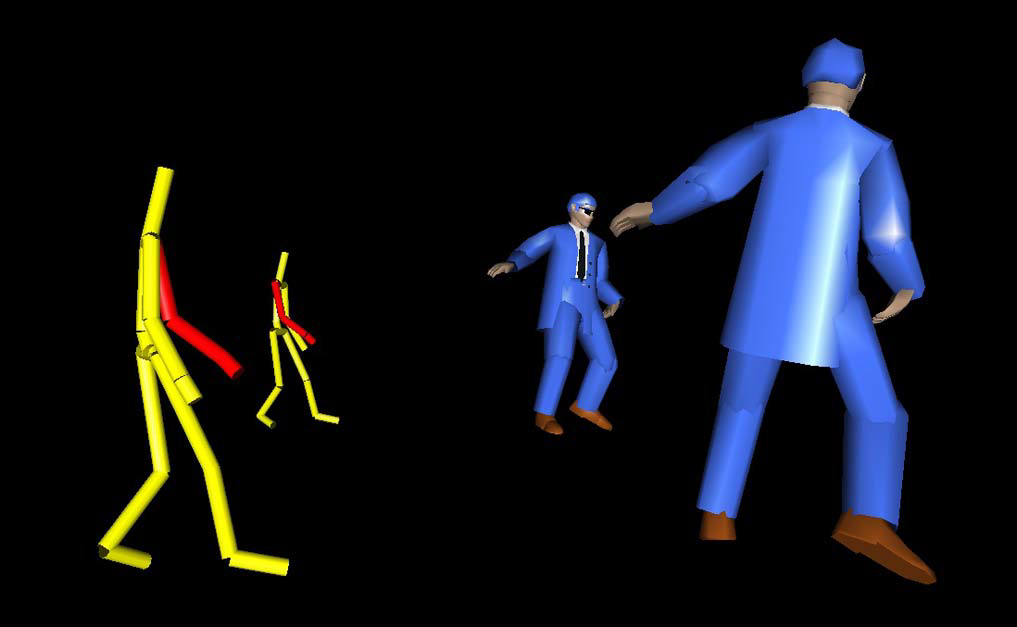
\includegraphics[width=0.45\textwidth]{img/VRDanceTrainerPractice.png}
	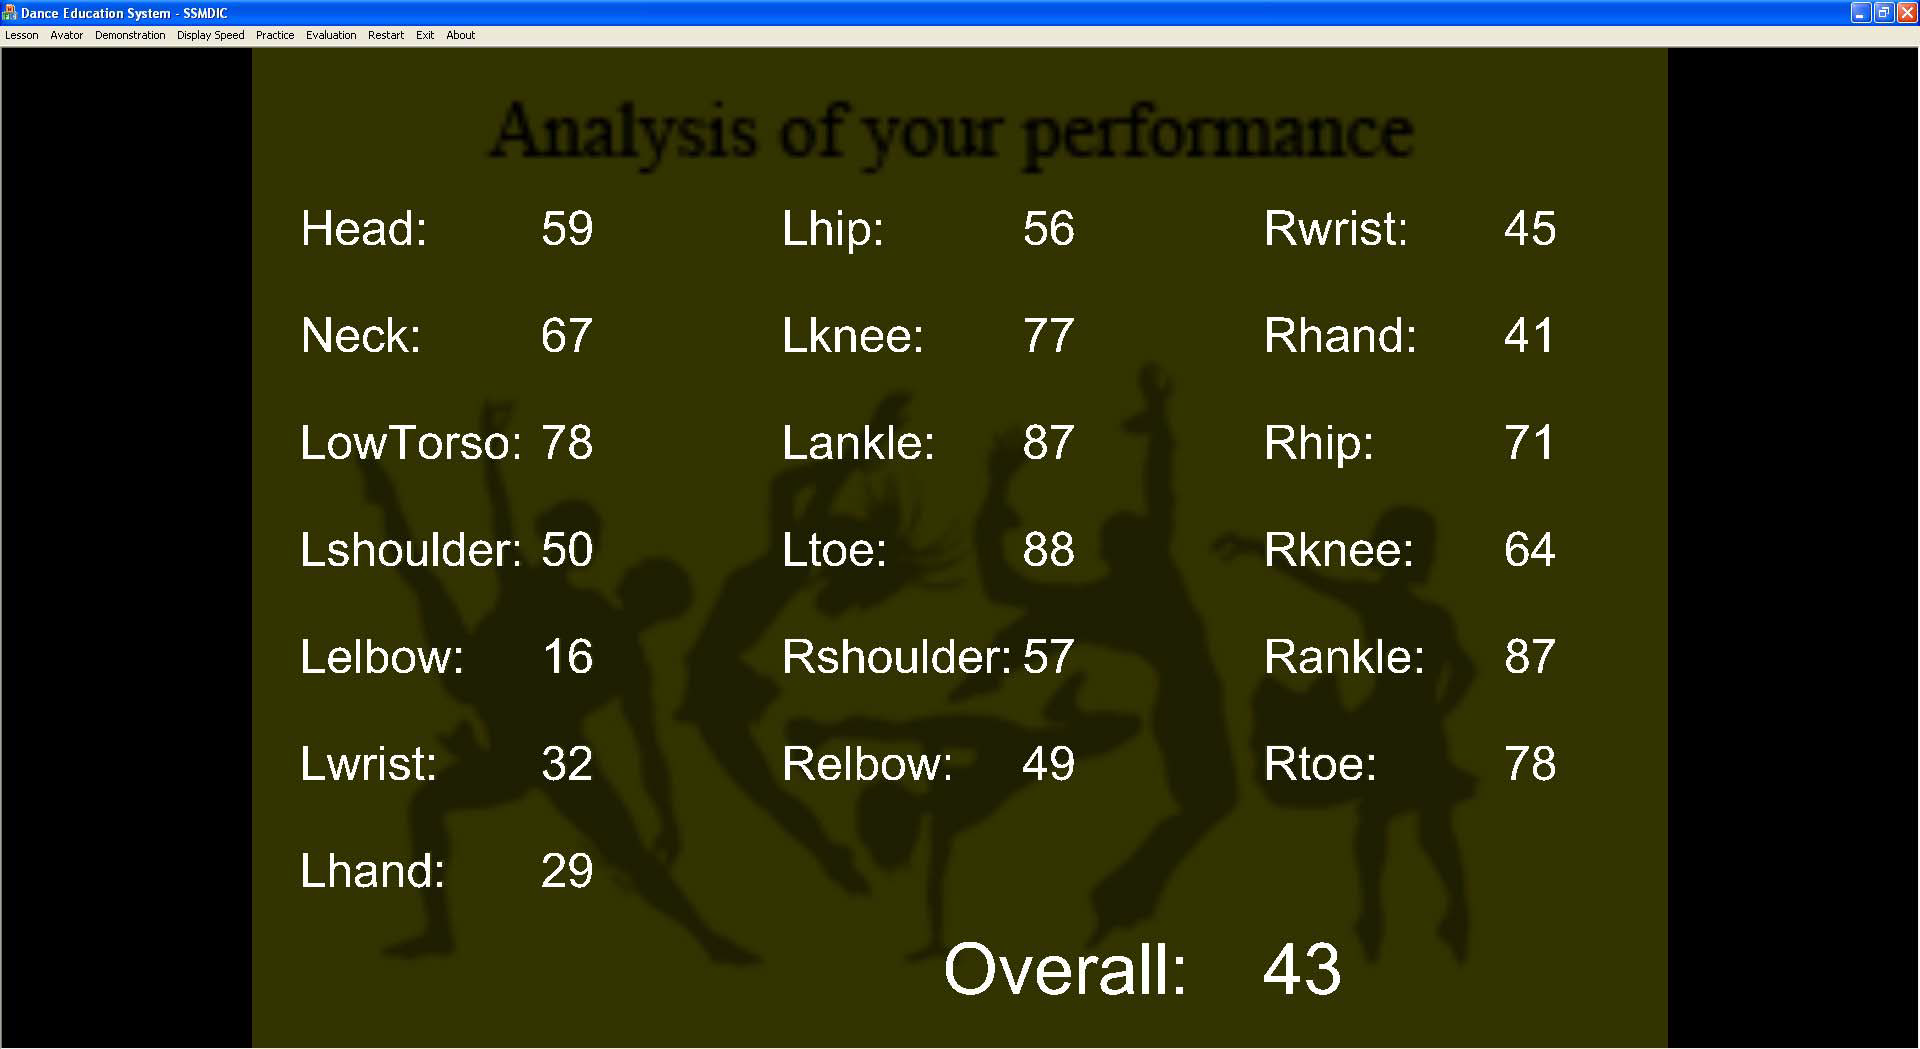
\includegraphics[width=0.5\textwidth]{img/VRDanceTrainerScoreBoard.png}
	\caption{\todo \cite{Chan2011a}}
	\label{fig:vrdt}
\end{figure}
%---
%visual appearence --- shape and colour
%gudance technique
%feedback
%realism degree
$ $\\
LightGuide \cite{Sodhi2012} compare six guidance visualisations:
\begin{itemize}
	\item Follow Spot: Moving light spot with elevation information. System sets pace.
	\item 3D F-Arrow: 3D arrow indicates the direction to move. System sets pace.
	\item 3D SG-Arrow: 3D arrow indicates the direction to move. User sets pace.
	\item 3D Pathlet: a line indicates the direction to move next. Current position indicated by a red spot.System sets pace.
	\item Video on hand: Instruction video projected on the hand. User sets pace.
	\item Video on screen: Traditional instruction video .User sets pace.
\end{itemize}
The main idea behind a guidance visualisation directly on the students body itself, is that the student can concentrate on the bodypart in question and not share the  with a instruction medium. The last condition proofed to be better than the second last, supporting this theses.
The student gets instant feedback by comparing the indicators with the hand. A larger offset results in increased indication in real time.\\ \\
%---
\textbf{OneBody} \cite{Hoang2016} use low realism degree avatars. Both, the student and the teacher are visualised by stick figures. The teachers avatar is red, the students avatar is blue. For feedback, if the students joints are matching joints of the teacher, these joints turn from blue to green, like shown in figure \ref{fig:ob1} left. Figure \ref{fig:ob1} right shows the scene from the first person perspective.
\begin{figure}
	\centering
	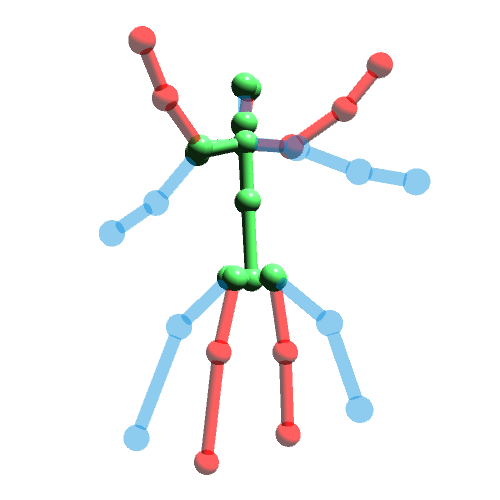
\includegraphics[width=0.225\textwidth]{img/onebody1.png}
	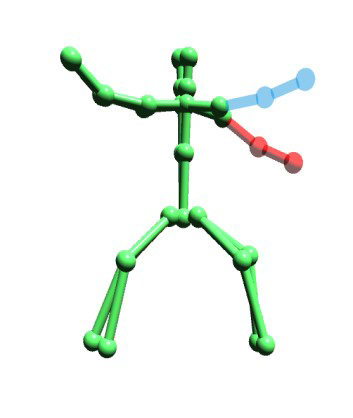
\includegraphics[width=0.225\textwidth]{img/onebody2.png}
	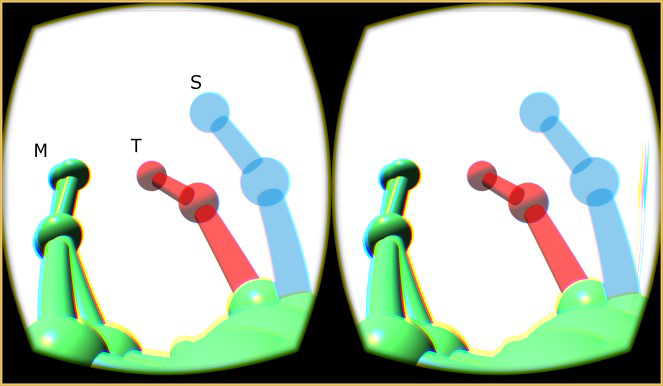
\includegraphics[width=0.45\textwidth]{img/onebody3.png}
	\caption{Left: student avatar (blue) and teacher avatar (red). Green limbs are matching limbs. Right: students view on the scene.\cite{Hoang2016}}
	\label{fig:ob1}
\end{figure}
The guidance itself takes place in real time. The remote teacher can give instructions by performing the postures and additionally verbally. The student mimics the postures and can compare his own joint positions with the positions of the teacher to correct the own joints. Hoang et al. compare the performance of the students achieved in Onebody with the performance in three other systems, namely with traditional video based learning, video conferencing and a 3rd person perspective in VR. The latter is very similar with Onebody but the teacher stands in front of the student. The system differe in exactly one aspect to each other, see figure \ref{fig:ob2}.
\begin{figure}
	\centering
	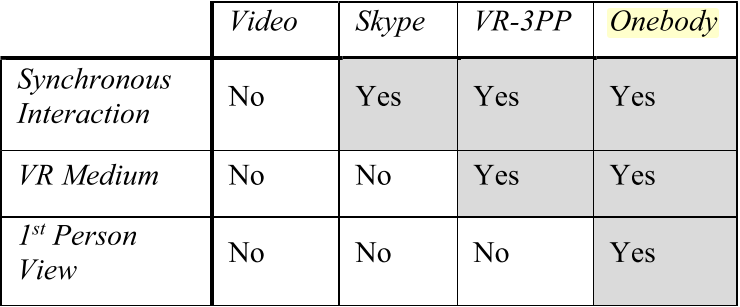
\includegraphics[width=0.5\textwidth]{img/onebody_training_methods.PNG}
	\caption{Training methods and their differences used in the study to evaluate Onebody \cite{Hoang2016}}
	\label{fig:ob2}
\end{figure}
%---
\textbf{Physio@Home} by Tang et al. \cite{Tang2015} use two guidance techniques. In the first, a video shows the movements instructions, the second they called "the wedge". The latter is a 3D plane showing the way of movement with direction indication. As feedback the current angle of the arm is shown. \todo figures
%---
%\subsection{Visual Appearance}
%\subsection{Degree of Realism}
%\subsection{Guidance Techniques}
%\subsection{Feedback}

\subsubsection{Conclusion}
The visual appearance of the guidance visualisations differ. The Tai Chi Trainer, YouMove, VR Dance Trainer and OneBody use person like avatars. These avatars perform a movement and the student mimics these movements. LightGuide and Physio@Home use direction indicators to visualise the movement in question. Movement indicators like arrows are less obtrusive for single body-part movements but become overwhelming for full body instructions. This work aims to analyse full body movements, therefore I choose here as visual appearance a person shaped avatar. The degree of realism of the avatar rage from stick figures to high realistic looking persons. Since Weber\todo showed a preference for realistic avatars I hereby choose high realism degree avatars as guidance visualisations. In addition, there is a difference in completion time based on the guidance technique. If the student sees the movement before hand completion time is significant lower. If the student grasp the movement by performing it, completion time is significant higher. A study must ensure that for all conditions the student could see the movement before performing the movement or not. Comparing with the real world, normally the student sees the movement before hand. This is why my study will provide this, too. Sodhi et al. state, that it is hard to compare self paced and system paced movements. To ensure comparability, only system paced movements will be evaluated. This ensures also only to evaluate precision of movements. In all systems feedback plays a role. Immediate feedback as well as aftermath feedback. For comparability, feedback must be consistent over all conditions. As Anderson et al. made clear, it is an important part for movement learning. This thesis does claim to provide full training system but an evaluation tool. For this reason only immediate feedback during learning will be provided. To ensure, that only the perspectives and not feedback is evaluated, exactly one and the same feedback method will be provided in all conditions. I choose here the overlay feedback without colour coding, where the student align his/her body with the body of the teacher avatar. Eventually, all authors point out the importance of scaling. To correctly match teacher and student, the teacher must be scaled to the students body.


\subsection{Dependent variables}
%---
In the Tai Chi trainer by Chua et al. \cite{Chua2003}, the students task is to mimic the motion of a pre recorded teacher. While the independent variables are the above mentioned perspectives (conditions a-e) and the motions, the independent variable is the precision of the performed movements. To measure this precision, twelve bones of the students were tracked, namely: upper and lower arms, hands, upper and lower legs, and feet. The bones are hierarchical structured with a parent and child end. After a normalization of the parents position and bone length, an error was calculated:
\begin{equation}
	\todo
\end{equation}
This error can be seen as the euclidean distance between the teacher's and the student's position of a bone. This error was calculated for every frame of the roughly 20 seconds with a rate of 60 fps:
\begin{equation}
	\todo
\end{equation}
The last four out of twelve trials were considered. So the measure of precision is described as:
\begin{equation}
	\todo
\end{equation}
This measure is an implementation of chapter 2 ref \todo.
Chua et al. found two major faults in this method of precision determination: yaw shift (\todo add in chapter 2 a definition of dofs) and time shift. To overcome the first, the initial position of the student was taken into account, the latter was fixed with a time frame comparison of 120 frames. Eventually this result was normalized with the difficulty (average number of errors per motion) of the motion task. This will be discussed in detail in the Projects Report. In addition, a post questionnaire was conducted where the students were asked to rate the difficulty of the representations. The results are discussed in the next section.\\ \\
%---
While Chua et al. calculate the error of the performed movement over all tracked limbs, Anderson et al. take one single joint with the greatest error and \--- even more constricting \--- only the keyframe joints (important joints, specified by the teacher) are taken into consideration. The dependent variable is a score between 0 and 10. An offset 15 cm results in a score of 7.5 and no error results in a score of 10. The offset is imply the eucledean distance. This error measurement corresponds to chapter 2 \todo. To overcome time shift errors, a window of 0.5 seconds is added. If the teacher specified that timing is important, this window is halved, if precision is set as important, 15cm offset results in a score of 7.5. "[]This values are determined by experimentation".\\ \\
%---
Chan et al. evaluate the students performance with the VR Dance Trainer. Therefore they specified 19 body parts (compare \ref{fig:vrdt} right) and calculate a score between 0 and 100. The average over the 19 numeric indicators results in the overall performance. Before and after the training session of one move this score was calculated. Additionally, a postcourse survey asked the student specific questions about the system. This survey had the aim to evaluate if the "[...] system is interesting and able to motivate subjects to learn." \cite{Chan2011a} and if the "[...] the system can provide them an easy way to learn" ibidem.\\ \\
%---
Sodhi et al \cite{Sodhi2012} compare in \textbf{LightGuides} evaluation the five conditions where the instruction in directly on the body of the user with a baseline condition where the instruction is on a screen. To measure the performance of the student, Sodh et al. developed two measures: movement accuracy and movement times. Movement accuracy describes the absolute euclidean distance from the closest point. Movement times is devided in two sections by the reason that half of the conditions were self timed and the half the pace was set by the system. For the self timed conditions the completion time is taken as measure, for system paced conditions the time before or after is taken as measure. Though, independent variable are the conditions, dependet variables are performance.\\ \\
%---
Hoang et al. \cite{Hoang2016} use six different measures to evaluate \textbf{Onebody}. \textit{Accuracy}, \textit{completion time}, \textit{instructors score}, \textit{ease to understand}, \textit{perceived precision} and \textit{preference}. For \textit{accuracy} the angles of limbs of the student and teacher were compared. This corresponds to \todo. For \textit{completion time} the time between start and "[...] the student feeling confident" was measured, but caps at 2 minutes. \textit{Instructors score} is a subjective score of the instructor after each posture. The data for the last three measures were gathered by post questionnaires. These scores were calculated for all four independent variables (video, video conference, 3rd person, Onebody)
%---
Physio@Home by Tang et al. \cite{Tang2015} use three performance measures to judge the students performance. Two distance measures, one for the elbow an one for the hand, and one angle measure for maximum of rotation. They ignored speed as a measure, because they were mainly interested in the precision of the movements. Additionally, two subjective measures were gathered: perceived accuracy and preference for method and preference for perspective.

\subsubsection{Conclusion}
All previous works use a performance measurement. These measurent varies but have a precision score in common. Some specify important body parts and give weights on these body parts. The error is measured in the eucledean distance. To overcome timing issues, an time frame between teachers and students movement apply. In addition, a second measurement is used: time. Completion time measures the time a student needs to feel confident to perform the movement. As subjective measurements, perceived accuracy and preference of method is widely used. Additionally OneBody asks the participants to judge the ease to understand. For my study I propose to implement a performance measure with a 0.5s time shift which proofed to be suitable. Furthermore, a completion time could give insights a objective perceived precision and speed of learning. As subjective scores, ease to understand, prefered method, perceived precision will be taken.

\subsection{Results}
%---
\textbf{Tai Chi Trainer}. Chua et al. compare different perspectives (conditions a-e) on the teacher and the student. The independent variables are the above mentioned precision of the students performance. By comparing the results they found condition a (One on One), b (Four Teachers), c (Side by Side) and e (Superimposition 2) aim the same precision. Only e (Superimposition 1) aimed significantly worse than the others. At the same time, the questionnaire indicated that the subjective difficulty of condition d and e (Superimposition 1 and 2) was the highest. "In fact, all of the subjects who tried Superimposition 2 thought it was the most difficult. Interestingly, although subjects considered Superimposition 2 very difficult compared to the other layouts, average error on that layout was not significantly greater than the other non-superimposed layouts." \cite{Chua2003}. The Authors argue this result as following:
\begin{itemize}
	\item simultaneously watching the teacher and performing own movements could interfere each other.\\
	Chua et al. suggests to choose wisely for the task to suit into VR training.
	\item latency and performance correlates strongly. A lower latency could lead to better performance.\\
	Since Chua et al. \cite{Chua2003} was developed in 2003, there is a large improvement in latency nowadays.
	\item To reduce latency a low polygon count on the high realism degree avatars was used. More polygons could lead to better performance.\\
	The system was run on a Pentium 3 processor. Today's graphic cards and processors are way above this mark, a higher polygon count is easily achievable.
	\item The field of view was very small.\\
	Today's VR HMDs probably provide a higher field of view (e.g. HTC Vive, 110$^\circ$).
\end{itemize}
%---
Anderson et al. compared \textbf{YouMove} with traditional video training, resulting in the independent variables \textit{YouMove} and \textit{Video}. The study was conducted with eight participants in a two factor repeated-measures design. Each participant had one ballet and one abstract task with both conditions. \textit{YouMove} scored significantly better than \textit{Video} by a factor of 2. \todo: elaborate a little bit more.\\ \\
%---
Chan et al. investigated three topics with the \textbf{VR Dance Trainer}. First the learning outcome, to proof if the student really got better with the system. Second, the "Arousing Interest" to inversigate weather the system motivates the students to learn. Eventually they compared the system with a traditional Self-leraning method. Comparing the the baseline score befre a training with the VR Dance Trainer with the score after the training session proofed a significant better performance. The post survey is interpreted by the authors with "Overall speaking, the subjects enjoy learning dance with our proposed system." ibidem. To compare the system with a traditional learning method, a control group conducted the same study only with the demonstration and no feedback. The basline scores showed no significant difference between the two groups but the post training scores did. Questionable remains, if a recording of a professional dancer rendered as an high realism degree avatar on a 3D screen can be called a traditional dance learning method.\\ \\
%---
Main finding of Sodhi et al. while evaluating \textbf{LightGuide} is an 85\% higher accuracy of ego-centric on body projections compared to a exo-centric video instructions.
Per student 90 datasets are generated (6 conditions x 5 path x 3 angles). The performance measure they applied, the conditions scored (best to worst): Follow Spot $<$ 3D F-Arrow $<$ 3d G-Arrow $<$ 3D Pathlet $<$ Video Hand $<$ Video Screen. Especially the relation between video on screen and video hand shows the importance of attention during guidance instruction. The instruction on the bodypart it self scored better than seeing the instruction on a screen. In terms of \textit{movement times}, both video conditions lead to lower movement times. Sodhi et al. see the reason therefore, that it makes a difference if the student sees the whole path before hand than or figuring out the movement as they moved along. Additionally, in an interview, participants of the study stated that self paced guidance are subjectivly like more than system paced. For system paced movement speed 30mm per second scored best in an pilot test. Further they suggest to plan regular recovery rests to exclude fatigue effects.\\ \\
%---
\textbf{Onebody} \cite{Hoang2016} proved to be significantly better over the other training measures in terms of \textit{accuracy}. Interestingly, no significant difference was found between the exo-centric 3rd person view and video conference. On the same time Onebody has a higher \textit{completion time} than the other systems. The instructors score showed no significance between the methods. Valuable for this work is, that the ego-centric perspective seems to be slightly better to \textit{understand} than the exo-centric perspective, but not significant. But both, ego and exo centric perspectives, are significantly harder to understand that the video based methods. Furthermore, the \textit{perceived precision} ego-centric perspective is significantly higher than the exo-centric perspective, but nearly on the same level as the video conference method. Eventually, Onebody is more \textit{preferred} by the participants of the study than 3rd person view. Hoang et al. conclude "[...] that synchronous training and 1st person view have a positive effect on posture accuracy." If this applies also to movements could be interesting to investigate.\\ \\
%---
\textbf{Physio@home} by Tang et al. \cite{Tang2015} investigated two subjective measures. The perceived accuracy ranked videoSingle < videoMulti < WedgeSingle < wedgeMulti. For the preferred method aimed for no clear preference. The study results show a higher performance with the multi view perspectives and also the wedge visualisation. The wedge visualisation in combination with multi view perspective achieved the highest performance. The authors see the reason in the ability to grasp the correct angle is much easier with the multi view perspective. Furthermore, the "corrective" feedback of the wedge encouraged the participants to correct themself. Tang et al. further state, that visualisations should contain as least as necessary information to not overwhelm the practitioners. 
\subsubsection{Conclusion}
LightGuide showed that ego-centric guidance performed better than exo-centric. On reason they see in the shift of attention. When the student can focus on the body part which is to move itself, the non shared attention plays a positive role in learning outcome. The ego-centric OneBody system proofed to be better that the exo-centric perspectives. Since OneBody only evaluates posture guidance, it could be interesting to find out if this also applies for movement guidance.



\section{conclusion}
In the scenario of one student learning from one teacher there are five main perspectives that can be thought of, excluding multiple copies of the teacher or the student on different positions. Tai Chi Trainer overcome the view angle issue with multiple copies, but I decided to tackle the issue by letting the student move freely around the teacher, like he could in the real world. This gives addditionally the possibility to observe how a student interacts with the virtual avatar, e.g. he walks side by side to extinct the right/left confusion while standing in front of the avatar. Comparing with figure \ref{fig:perspectives} 1. is the ego-centric perspective, here the teacher stands inside the student. 4. is closest to the real world, where a teacher stands in front of the student, representing an exocentric view. But as we found above, by standing the teacher inside the student, the student can align his body with the teacher. This is a form of feedback, because missplacement is easy to see. 1. thereby has feedback and 2. don't which makes it hard to compare. 2. is a exo-centric view on the teacher and the student stands inside of the teacher, providing a similar feedback to 1. what maintains the comparability of these two perspectives. 3. is the combination of the ego-centric perspective and the exo-centric perspective. The student sees the teacher in front of him and inside of him. Consequently, 5. is also ego-centric and exo-centric. The teacher standing in the student and the student in the teacher provides double feedback.\textbf{ Max, hier müssen wir uns für die perspectiven entscheiden.}\\ \\
\begin{figure}
	\centering
	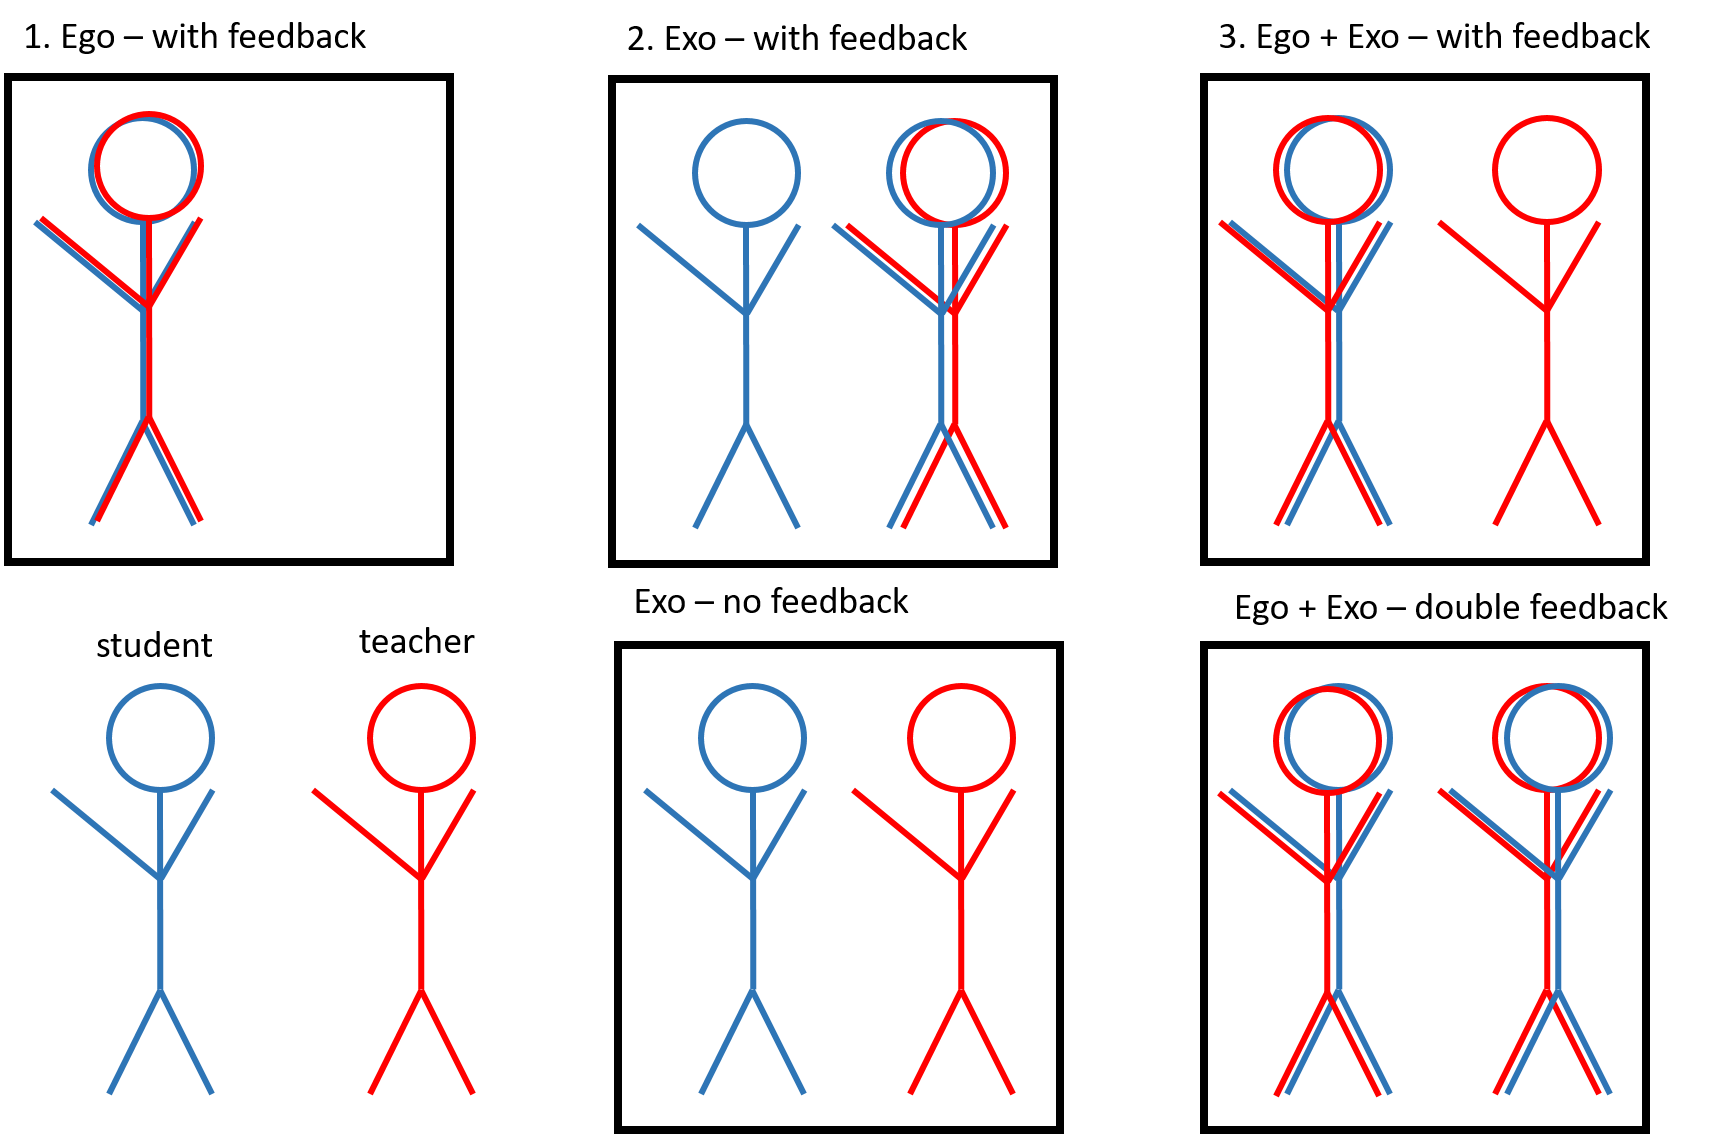
\includegraphics[width=1.0\textwidth]{img/perspectives.png}
	\caption{possible perspectives}
	\label{fig:perspectives}
\end{figure} \\ \\
abschließende worte...

\begin{comment}

%----------------------------------------------------
\begin{comment}
\section{in detail - Onebody: Remote Posture Guidance System using First Person View in Virtual Environment}

Onebody by Hoang et al. \cite{Reinoso2016} is a VR system for remote posture guidance. 
%Onebody is designed for sports or physical activity training like yoga, dance or martial arts.
The student and the teacher are both tracked by skeletal tracking. The visualisation of this tracking are shown via a VR headset, allowing the student to follow the instruction of the teacher in first person view of the teacher - which means the student "stands inside the body of the teacher". 


When the teacher moves his limbs, the student can see the movement emerging from himself. Now the student can move his own limbs to mimic the movement till the teachers posture is matched. The teacher sees the students limbs likewise allowing him to give instant feedback to the student. Thus, "Onebody provides a medium to deliver body movement instructions for non-collocated instructor and learner." \todo. %The visualisations are attached to the hip but keeps the mapping between the user and corresponding avatar. To overcome different body sizes, the avatars are normalised and scaled to the size of the person seeing the avatars.\\
For transfering data, both the teacher and the student are clients in a server-client system. The clients are sending the their tracking data to the server which is broadcasting it to the clients. The comparison of the limbs for colour coding is performed on the client side. The matching of the limbs is calculated by the position of the single limbs (see equation \eqref{eq:constanterror}) with a threshold of 5cm to reduce jitter and tracking errors. Limbs in question are wrist, elbow, shoulder, hip, knee and ankle. The feedback with colour codes is provided in realtime.\\
With this system hoang et al. designed a user study to evaluate the performance of posture accuracy and user's preference. Their main hypotheses is "\textit{Onebody delivers better posture accuracy than existing remote movement instruction methods}". "Posture accuracy is determined by the extend to which the student can replicate the final posture as instructed and demonstrated by the instructor." In addition, completion time and a subjective score of the instructor are considered.
To test the hypothesis, Onebody was compared with three other remote posture training methods (independent variables): pre recorded video, video conference (Skype), VR 3rd person perspective. Each of the systems differs to Onebody in terms of synchronous interaction, VR medium and perspective see figure \ref{fig:ob2}.

%The study was a 4x4 within subject. Each participant stated with a training session in which the not collocated instructor teach a posture physically and verbally. Verbal feedback was given the training repeated until the student was confident. After that the final posture was recorded. A set of four of postures with every system were performed with different complexities.\\
The results show a significant difference in accuracy. Onebody performed significantly better in over video conference, 3rd person VR and pre recorded video. Furthermore, the completion time was significantly higher with Onebody as in the other three systems. The subjective score of the instructor showed no significant differences. A post questionnaire indicated that Onebody is harder to understand and use than the other systems, but at the same time it also indicated that Onebody was perceived to be more exact. Participants rated video conference as their most preferred system over Onebody and 3rd person VR.
%--------

Researchers utilised the theory of the last chapter to design MR Motor Learning systems in various ways. They differ in the technology, tasks, perspectives measures etc. In this chapter we analyse these systems to extract valuable insights to design a MR Motor learning System. First we analyse the aspects of MRML systems. After that we take a close look on some systems how they conducted their investigation and their outcome.

\section{Aspects of MR Motor Learning systems}
paper to come:
\begin{itemize}
	\item Cruz: Cyclone uppercut
	\item Davcev: AR Environment for Dance Learning
	\item Chan: Immersive Performance training Tools Using Motion Capture Technology
	\item Han: AR-Arm: Augmented Visualization for Guiding Arm Movment in the First-Person Perspective
	\item han: My Tai-Chi Coaches: An Augmented-Learning Tool for Practicing Tai-Chi Chuan
\end{itemize}

\subsection{Method}
Jacky Chan et al. \todo created a VR dance training system using an optical motion capturing system to compare the movements performed by the student with movements from the avatar. These movements are presented to the student as a 3D rendering on large screen. The movements of the students are visualised on the same screen as a coloured stick figure. The student mimics these movements and gets instant feedback as well as a feedback as a summary.

In contrast, Onebody by Hoang et al. \todo use a VR headset for a first person remote posture guidance system. 

\subsection{Tasks}
In Chan et al. \todo the dance student is presented a virtual avatar performing dance moves of A-go-go or Hip-Hop style. The avatars movement is based on the motion capturing data of a professional dancer. Onebody \todo is not only restricted to dance moves but also include other posture based sports or physical activities like Yoga or Mixed Martial Arts.

Onebody \todo uses a number of martial arts postures or stances.
\begin{itemize}
	\item Onebody: 16 artificial postures not from but like: tai chi, matial arts
	\item VR Dance Trainer: dance movements, 15 min for each move
	\item you move: various movements to perform. using a whip, baseball, boxing, ballet, dance moves
	\item training archived physical skills IVE: physical skills in sport activities, especially baseball pitching
\end{itemize}

\subsection{Measures and variables}
Jacky Chan et al. \todo defined 19 body parts that are considered in the measure of the performance of the dancing student. They name three features to compare the difference between two motions common: joint position, joint velocity and joint angle. Chan investigated which of these features suits most to judge the two dancing motions. The outcome of this investigation names the joint position to have the highest discriminative power. Hence, the joint position suits them best for their evaluation, Chan et al. calculate a score of the position error for each of the defined body parts, as well as an overall score. 

Onebody \todo uses skeletal of the instructor and the student
"Posture accuracy is determined by the extend to which the student can replicate the final posture as instructed and demonstrated as by the instructor." Independent variable: mothods for posture training. dependent variables: performance factors of posture accuracy, completion time, subjective instructor rating, users preference.

\begin{itemize}
	\item scientific work, how to measure movements: hachimura et al, yoshimura et al, qian et al, kwon et al, all use joint angles,  (mentioned in: vr dance trainer)
	\item onebody: skeletal tracking, how much percent do the postures match? 3d positions of limbs measured: wrist, elbow, shoulder, hip knee ankle. so angle between bones is the main measure for accuracy. additionally a subjective instructor score was recorded. And, completion time, topped by 2 min.
	\item VR Dance trainer: there are 3 common features for measuring hte difference between movements: joint position, velocity, angle. they tested which feature descibes movements best: joint position. base line vs post training movements are compared.
	\item you move: in each keyframe, score based on the joint with the maximum error, measured in euclidean distance. but only "important joints" are measured. timing errors: 0.5s error on each side of the frame for matching posture. is timing important, the window is reduced to 0.25s. max eucl. distance is linear mapped to a score. 0 error is 10 (max), 10cm is 7.5 what is the score to pass. if precision is important, 10cm needed for pass.
\end{itemize}

\subsection{Considered Body Parts}
scientific work, how to measure movements: hachimura et al, yoshimura et al, qian et al, kwon et al, all use joint angles

error prevention \todo

\section{Detailed description of 6-10 papers incl. Table}
%hier werden die paper detailiert vorgestellt von denen ich dann meine tasks, measures, methode und variablen ableite. am ende zusammenfassung in einer tabelle






\section{Research Gap}
lücken in der aktuellen forschung die sich lohnen zu untersuchen. \todo

\subsection{Conclusion of VR motor learning systems}
to conclude we have a look a Table \ref{table:ConclusionVRSystems}
\begin{table}[]
	\begin{tabular}{|l|l|l|l|l|l|}
		\hline
		Name & Hardware & Perspectives & Task & Measures & Variables \\ \hline
		Onebody &  &  &  &  &  \\ \hline
		VR dance trainer &  &  &  &  &  \\ \hline
		&  &  &  &  &  \\ \hline
		&  &  &  &  &  \\ \hline
		&  &  &  &  &  \\ \hline
		&  &  &  &  &  \\ \hline
	\end{tabular}
	\caption{Summary of proposed MR learning systems}
	\label{table:ConclusionVRSystems}
\end{table}


Research questions?\\
Hypothesis?\\
\end{comment}